\chapter{Simulazione di una coda $M/G/1//Prio$}

\section{Sistema a coda $M/G/1//Prio$}


Per la simulazione di un sistema a coda con classi di priorit\`a assegnata agli utenti \`e possibile, attreverso l'opportuna scheda, selezionare le varie configurazioni per la caratterizzazione delle classi.

Tali configurazioni comprendono, in aderenza alle specifiche fornite, due o tre classi alle quali sono associate differenti priorit\`a. Per la specificit\`a delle stesse si rimanda alla tabella \ref{tab:mg1prioclasses}.

\begin{table}[!h]
	\begin{center}
	\begin{tabular}{|ccl|}
	\hline
	ID  & n. classi & caratteristiche\\
	\hline
	2 & 2 & $\rho_{1}=x\rho$  \\
	& & $\rho_{2}=(1-x)\rho$ \\
	\hline
	3a & 3 & $\rho_{1}={x\over2}\rho$  \\
	& & $\rho_{2}={x\over2}\rho$  \\
	& & $\rho_{3}=(1-x)\rho$  \\
	\hline
	3b & 3 & $\rho_{1}={x\over10}\rho$ \\
	& & $\rho_{2}={9x\over10}\rho$  \\
	& & $\rho_{3}=(1-x)\rho$  \\
	\hline
	3c & 3 & $\rho_{1}=x\rho$ \\
	& & $\rho_{2}={(1-x)\over2}\rho$  \\
	& & $\rho_{3}={(1-x)\over2}\rho$  \\
	\hline
	\end{tabular}
	\end{center}
	\caption{Caratteristiche delle configurazioni di classi disponibili.}
	\label{tab:mg1prioclasses}
\end{table}

\begin{figure}[!h]{
	\begin{center}
	   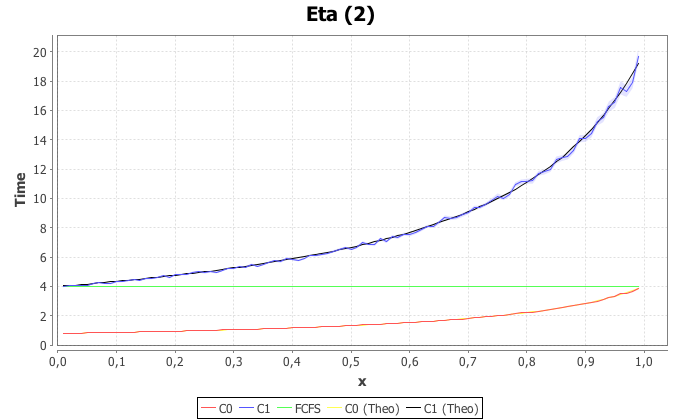
\includegraphics[width=\textwidth]{figures/MG1PRIO[2,mu1,r10000].png}
	\end{center}}
	\caption{Tempi medi di attesa medio nel sistema con coda a due classi di priorit\`a}
	\label{fig:mg1prio2}
\end{figure}

Analogamente a quando disposto nel caso della simulazione di sitema di tipo $M/G/1$, al termine dell'elaborazione verranno visualizzati i risultati grafici relativi alla simulazione svolta.

Nello specifico, la variabile $x$ viene fatta variare all'interno dell'intervallo (0,1), precedentemente suddiviso in $100$ quanti.

Gli andamenti degli $\overline{\eta}$ relativi alle varie classi mostrati all'interno dei grafici sono contraddistinti da una particolare notazione grafica che, attraverso l'utilizzo della medesima colorazione assegnata alla rispettiva classe, evidenzia gli intervalli di confidenza senza rendere difficoltosa l'interpretazione dei grafici, come invece accadrebbe con l'usuale notazione degli stessi.

Le diverse caratterizzazioni delle classi di priorit\`a, definite come da specifica richiesta, sono consultabili in tabella \ref{tab:mg1prioclasses}.


\begin{figure}[!h]{
	\begin{center}
	   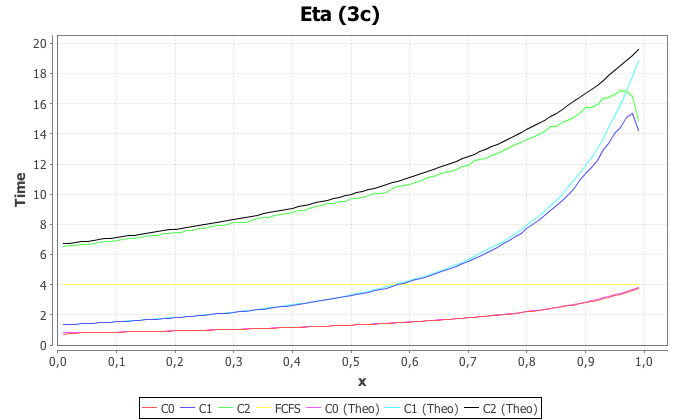
\includegraphics[width=\textwidth]{figures/MG1PRIO3c[mu=2,runs=10000,arrivals=1000].png}
	\end{center}}
	\caption{Tempi medi di attesa nel sistema con coda a tre classi (tipo c)}
	\label{fig:mg1prio3c}
\end{figure}


\begin{figure}[!h]{
	\begin{center}
	   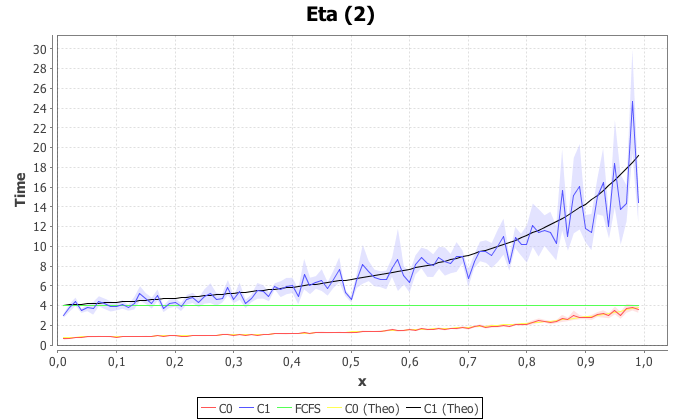
\includegraphics[width=\textwidth]{figures/mg1prio2low.png}
	\end{center}}
	\caption{Tempi medi di attesa nel sistema con coda a due classi (basso \#runs)}
	\label{fig:mg1prio2low}
\end{figure}

\subsubsection{Nota}

Nei grafici mostrati in figura \ref{fig:mg1prio2} e \ref{fig:mg1prio3c} non \`e possibile apprezzare a pieno gli intervalli di confidenza a causa della specificit\`a dei test eseguiti. In particolare le simulazioni relative alle suddette figure sono state compiute con quantit\`a di dati parcolarmente elevate, che  hanno determinato un'apprezzabile precisione dei risultati oltre ad una notevole durata in termini di tempo di simulazione. \\ Dualmente, la figura \ref{fig:mg1prio2low} \`e il risultato di una simulazione a due classi di priorit\`a effettuato specificando un numero molto inferiore di \emph{runs} e \emph{arrivi}, in maniera tale da mostrare l'incertezza dovuta alla discordanza tra i risultati: in particolare nell'immagine \`e possibile notare, che contorna ciascuna delle due linee, un'ombratura particolare che meglio identifica l'intervallo di confidenza puntuale associato al valor medio di $\eta$ al variare di $x$. 

\subsection{Analisi tecnica}

Anche in questo caso per l'implementazione della simulazione sono state seguite le linee guida presenti nella documentazione del corso. Il corpo della simulazione, definito all'interno della classe {\tt SimulatorRunners} (si veda fig \ref{fig:simulatorclass}), \`e suddiviso in una prima parte di parsing dell'input fornito dall'utente (metodo {\tt simulateMG1PrioWithVariableRhos(...)} durante il quale si definiscono i valori di $\rho_{1,2,(3)}$ e quindi dalla simulazione vera e propria, implementata all'interno del metodo {\tt simulateMG1Prio(...)}.

Tale metodo si appoggia sulla concretizzazione della classe astratta {\tt Simulator}, {\tt FCFSSimulator}, in cui si implementa un simulatore di tipo singolo servitore, con pi\`u code di attesa a decrescente grado di priorit\`a, ciascuna ordinata in base al semplice tempo di arrivo, {\tt OccurenceTime}. \\ Si vuole qu\`i inoltre notare che i singoli eventi che accadono all'interno del simulatore (arrivi e partenze) vengono mappati in analoghe classi ({\tt Event}, {\tt Arrival} e {\tt Departure} rispettivamente) organizzate in una gerarchia che vede sia gli arrivi che le partenze come specializzazioni del generico (e astratto) evento. Inoltre, come scelta progettuale, si \`e deciso di non includere nei singoli eventi anche la relativa politica di ordinamento, che viene invece specificata di volta in volta in classi appositamente create, derivanti da {\tt ComparableEvent}, le quali fungono da \emph{wrapper} dello specifico evento e ne stabiliscono i criteri di ordinamento; nel caso in questione una particolare sottoclasse di {\tt ComparableEvent}, {\tt OccurrenceTimeComparedEvent}, stabilisce, come politica, un ordinamento semplicemente basato sul tempo di occorrenza dell'evento: \emph{first-come-first-served}.









